\documentclass[aspectratio=169,10pt]{beamer}

\usetheme{Madrid}
\usecolortheme{seahorse}

\usepackage[utf8]{inputenc}
\usepackage{amsmath}
\usepackage{amssymb}
\usepackage{amsfonts}
\usepackage{xcolor}
\usepackage{listings}
\usepackage{graphicx}
\usepackage{hyperref}
\usepackage{cancel}

% Configure listings for code
\lstset{
  basicstyle=\ttfamily\scriptsize,
  breaklines=true,
  commentstyle=\color{green!50!black}\itshape,
  keywordstyle=\color{blue},
  stringstyle=\color{red},
  showstringspaces=false,
  numbers=left,
  numberstyle=\tiny,
  frame=single,
  captionpos=b,
  language=python
}

% Set graphics path
\graphicspath{{figures/}}

% Configure footer
\setbeamertemplate{footline}[frame number]

% Title slide
\title[Ch. 15: Fenchel-Rockafellar Duality]{Chapter 15: Fenchel-Rockafellar Duality}
\author{Convex Analysis and Monotone Operator Theory}
\date{2024}
\institute{Based on: Convex Analysis and Monotone Operator Theory in Hilbert Spaces (2e, 2017)}

\begin{document}

\frame{\titlepage}

% ============================================================================
% SECTION: Introduction and Overview
% ============================================================================

\section{Introduction}

\begin{frame}{Chapter 15 Overview}
  \begin{enumerate}
    \item \textbf{15.1:} The Attouch-Brézis Theorem
      \begin{itemize}
        \item Exact formula for sum of conjugate functions
        \item Infimal convolution properties
      \end{itemize}
    
    \item \textbf{15.2:} Fenchel Duality
      \begin{itemize}
        \item Primal-dual optimization problems
        \item Duality gap and optimality conditions
      \end{itemize}
    
    \item \textbf{15.3:} Fenchel-Rockafellar Duality
      \begin{itemize}
        \item Duality with linear operators
        \item Zero duality gap conditions
      \end{itemize}
    
    \item \textbf{15.4:} A Conjugation Result
      \begin{itemize}
        \item Conjugate of composite functions
      \end{itemize}
    
    \item \textbf{15.5:} Applications
      \begin{itemize}
        \item Von Neumann's minimax theorem
        \item Convex cone and operator results
      \end{itemize}
  \end{enumerate}
\end{frame}

\begin{frame}{Key Concepts}
  \textbf{Fenchel Conjugate:}
  For $f: \mathcal{H} \to [-\infty, +\infty]$,
  \[
    f^*(u) = \sup_{x \in \mathcal{H}} \left( \langle u, x \rangle - f(x) \right)
  \]
  
  \vspace{0.5cm}
  
  \textbf{Infimal Convolution:}
  For $f, g \in \Gamma_0(\mathcal{H})$,
  \[
    (f \text{ } \square \text{ } g)(x) = \inf_{y \in \mathcal{H}} [f(y) + g(x - y)]
  \]
  
  \vspace{0.5cm}
  
  \textbf{Primal-Dual Problem:}
  \begin{itemize}
    \item \textbf{Primal:} $\min_x [f(x) + g(x)]$
    \item \textbf{Dual:} $\min_u [f^*(-u) + g^*(u)]$
  \end{itemize}
\end{frame}

% ============================================================================
% SECTION 15.1: Attouch-Brézis Theorem
% ============================================================================

\section[15.1]{Section 15.1: The Attouch-Brézis Theorem}

\begin{frame}{The Attouch-Brézis Theorem}
  \begin{block}{Theorem 15.3 (Attouch-Brézis)}
    Let $f$ and $g$ be functions in $\Gamma_0(\mathcal{H})$ such that
    \[
      0 \in \text{sri}(\text{dom} f - \text{dom} g)
    \]
    where \texttt{sri} denotes the \textbf{strong relative interior}.
    
    Then:
    \[
      (f + g)^* = f^* \text{ } \square \text{ } g^*
    \]
  \end{block}
  
  \vspace{0.3cm}
  
  \textbf{Key Insight:} The conjugate of a sum equals the infimal convolution of conjugates under a constraint on domain difference.
\end{frame}

\begin{frame}{Illustration: Attouch-Brézis}
  \centering
  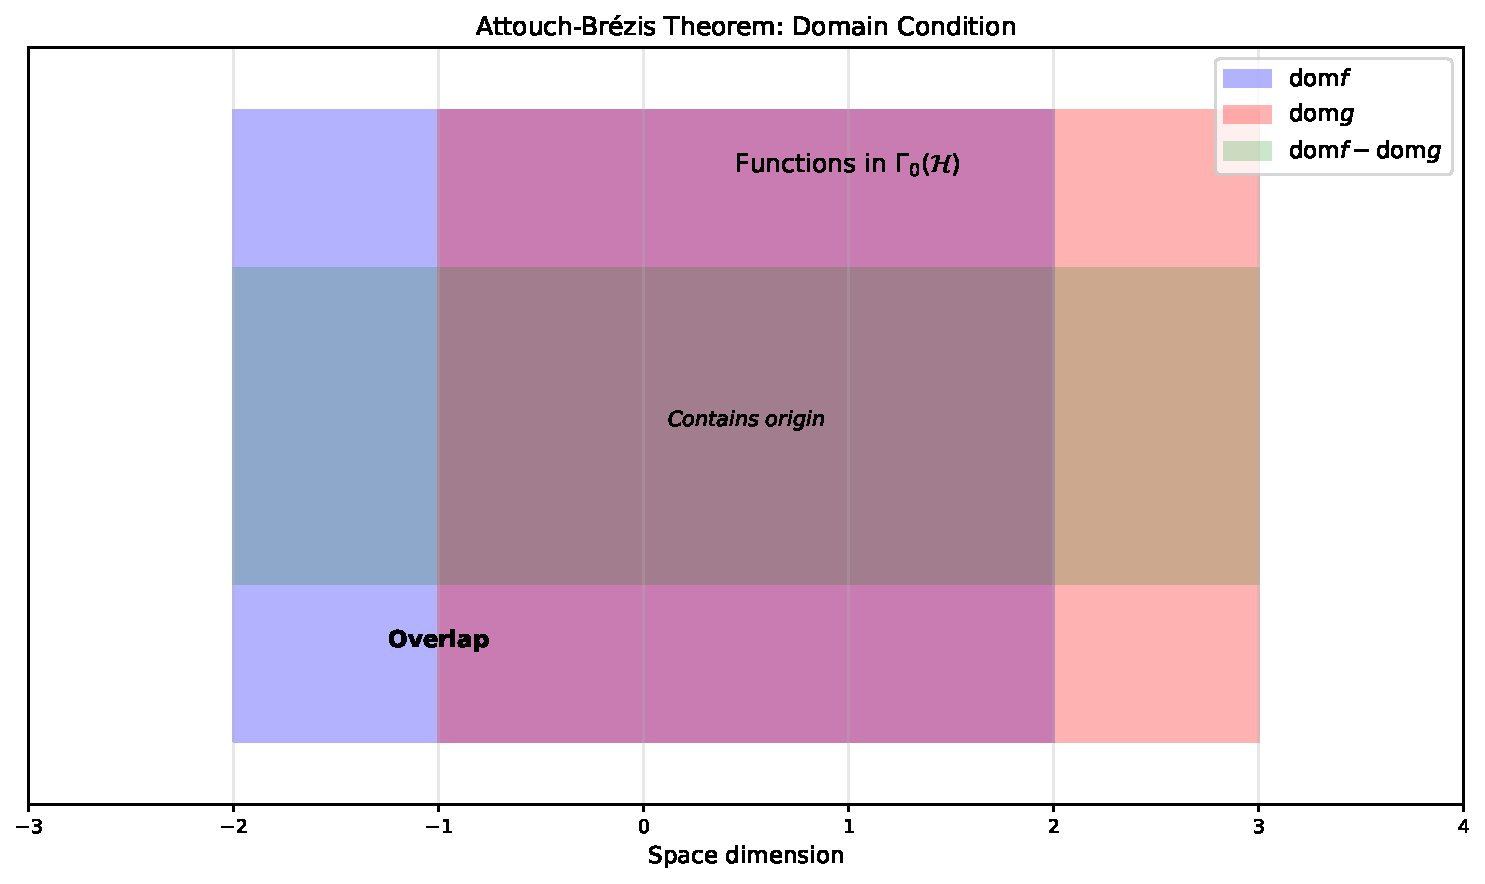
\includegraphics[width=0.9\textwidth]{attouchbrezis_illustration.pdf}
  
  \vspace{0.3cm}
  The condition $0 \in \text{sri}(\text{dom} f - \text{dom} g)$ ensures domains interact properly.
\end{frame}

\begin{frame}{Proposition 15.5: Sufficient Conditions}
  \begin{block}{Proposition 15.5}
    Let $f, g \in \Gamma_0(\mathcal{H})$ with $\text{dom} f \cap \text{dom} g \neq \emptyset$.
    
    Any one of these implies $0 \in \text{sri}(\text{dom} f - \text{dom} g)$:
    \begin{enumerate}
      \item[(i)] $\text{cone}(\text{dom} f - \text{dom} g) = \text{span}(\text{dom} f - \text{dom} g)$
      \item[(ii)] $0 \in \text{core}(\text{dom} f - \text{dom} g)$
      \item[(iii)] $0 \in \text{int}(\text{dom} f - \text{dom} g)$
      \item[(iv)] $\text{cont} f \cap \text{dom} g \neq \emptyset$
      \item[(v)] $\mathcal{H}$ is finite-dimensional and $\text{ri}(\text{dom} f) \cap \text{ri}(\text{dom} g) \neq \emptyset$
    \end{enumerate}
  \end{block}
\end{frame}

\begin{frame}[fragile]{Example: Attouch-Brézis Application}
  \textbf{Example:} Let $\mathcal{H} = \mathbb{R}$, $f(x) = |x|$, $g(x) = x^2 + 1$.
  
  \vspace{0.3cm}
  \textbf{Conjugates:}
  \begin{itemize}
    \item $f^*(u) = \begin{cases} 0 & \text{if } |u| \leq 1 \\ +\infty & \text{otherwise} \end{cases}$
    \item $g^*(u) = \frac{u^2}{4} - 1$
  \end{itemize}
  
  \vspace{0.3cm}
  
  \textbf{Computation of $(f+g)^*$:}
  \begin{lstlisting}
# Python example
import numpy as np
f = lambda x: np.abs(x)
g = lambda x: x**2 + 1
combined = lambda x: f(x) + g(x)

# The conjugate property holds when domains satisfy the condition
# (f + g)*(u) = inf_v [f*(v) + g*(u - v)]
  \end{lstlisting}
  
  The Attouch-Brézis theorem ensures exact conjugacy formula.
\end{frame}

\begin{frame}{Remark 15.4: Tightness of Conditions}
  \begin{block}{Key Remarks}
    \begin{enumerate}
      \item If $\mathcal{H} = \mathbb{R}^2$ and $\text{dom} f = \mathbb{R} \times \{0\}$, $\text{dom} g = \{0\} \times \mathbb{R}$, then
        \[
          (f + g)^* = \iota_{\{0\}} \quad \text{but} \quad f^* \text{ } \square \text{ } g^* \neq \iota_{\{0\}}
        \]
      
      \item Theorem 15.3 can fail if strong relative interior is replaced by relative interior.
      
      \item Lower semicontinuity of $f$ and $g$ is necessary.
    \end{enumerate}
  \end{block}
  
  These examples show conditions in Theorem 15.3 are tight and cannot be weakened.
\end{frame}

% ============================================================================
% SECTION 15.2: Fenchel Duality
% ============================================================================

\section[15.2]{Section 15.2: Fenchel Duality}

\begin{frame}{Fenchel Duality: Basic Framework}
  \begin{block}{Definition 15.10}
    For proper functions $f, g: \mathcal{H} \to [-\infty, +\infty]$:
    
    \textbf{Primal Problem:}
    \[
      \min_{x \in \mathcal{H}} [f(x) + g(x)]
    \]
    
    \textbf{Dual Problem:}
    \[
      \min_{u \in \mathcal{H}} [f^*(-u) + g^*(u)]
    \]
    
    \textbf{Duality Gap:}
    \[
      \Delta(f,g) = \begin{cases}
        0 & \text{if } \mu = -\mu^* \in [-\infty, +\infty] \\
        \mu + \mu^* & \text{otherwise}
      \end{cases}
    \]
    where $\mu = \inf(f+g)(\mathcal{H})$ and $\mu^* = \inf(f^* + g^*)(\mathcal{H})$.
  \end{block}
\end{frame}

\begin{frame}{Fenchel Duality Gap Analysis}
  \centering
  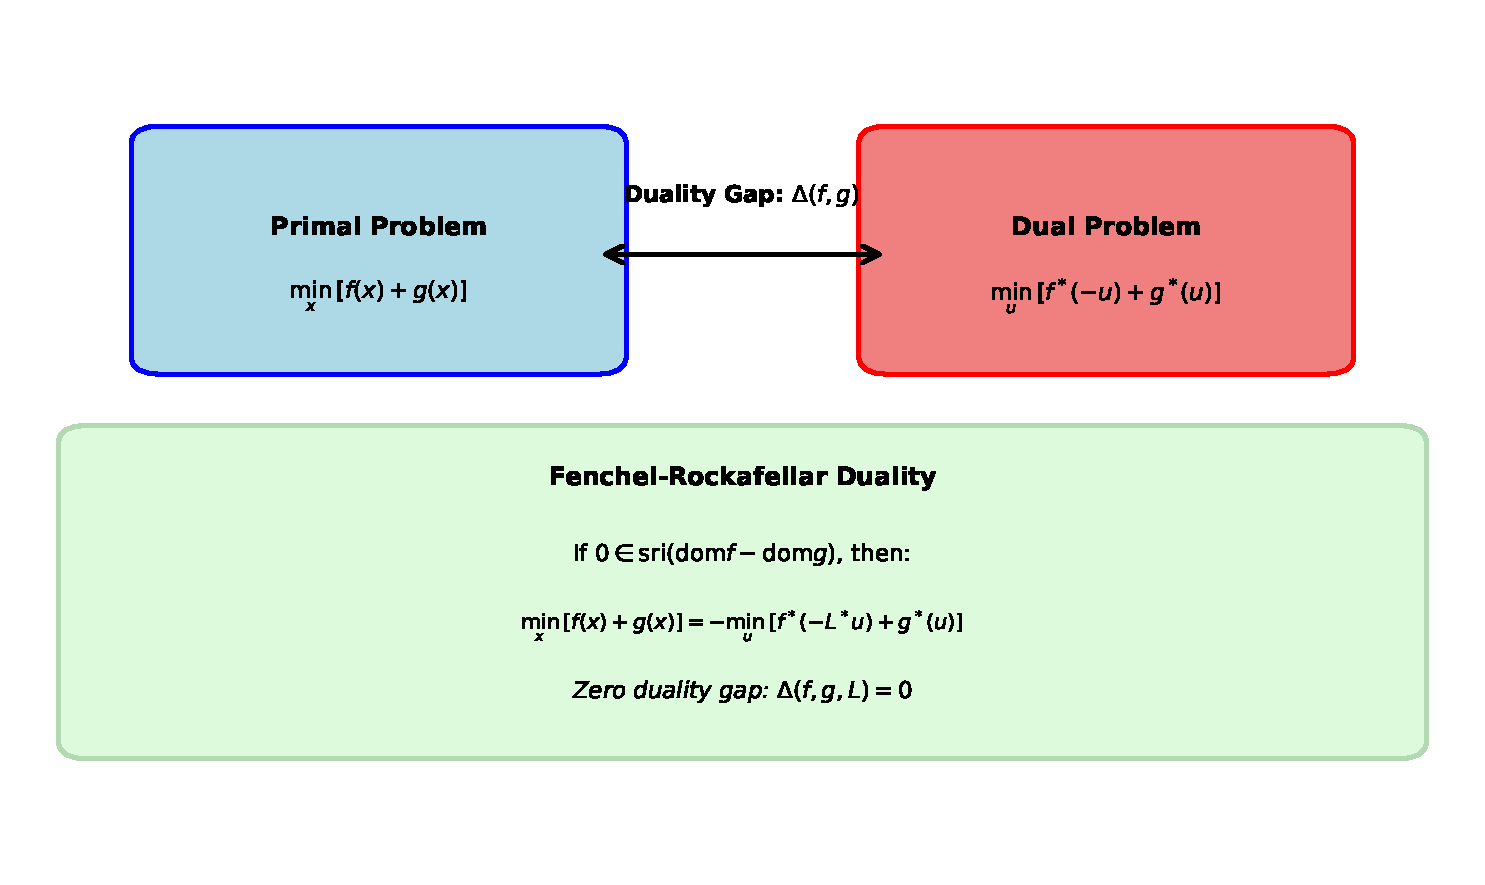
\includegraphics[width=0.85\textwidth]{duality_gap.pdf}
  
  The duality gap $\Delta(f,g)$ measures the difference between optimal values.
\end{frame}

\begin{frame}{Proposition 15.9: Weak Duality}
  \begin{block}{Proposition 15.9}
    For proper functions $f, g: \mathcal{H} \to [-\infty, +\infty]$:
    
    \[
      (\forall x \in \mathcal{H})(\forall u \in \mathcal{H}) \quad f(x) + g(x) \geq -f^*(-u) - g^*(u)
    \]
    
    Hence:
    \[
      \inf(f+g)(\mathcal{H}) \geq -\inf(f^* + g^*)(\mathcal{H})
    \]
  \end{block}
  
  \vspace{0.3cm}
  \textbf{Proof Sketch:} Using Fenchel-Young inequality:
  \[
    \langle u, x \rangle \leq f(x) + f^*(u) \quad \text{and} \quad \langle u, x \rangle \leq g(x) + g^*(u)
  \]
\end{frame}

\begin{frame}{Proposition 15.12: Duality Properties}
  \begin{block}{Proposition 15.12}
    Let $f, g$ be proper, and set
    \[
      \mu = \inf(f+g)(\mathcal{H}), \quad \mu^* = \inf(f^* + g^*)(\mathcal{H})
    \]
    
    Then:
    \begin{enumerate}
      \item[(i)] $\mu \geq -\mu^*$ \quad (weak duality)
      \item[(ii)] $\Delta(f,g) \in [0, +\infty]$ \quad (gap is non-negative)
      \item[(iii)] $\mu = -\mu^* \Leftrightarrow \Delta(f,g) = 0$ \quad (strong duality)
    \end{enumerate}
  \end{block}
  
  \vspace{0.3cm}
  Strong duality ($\Delta(f,g) = 0$) means optimal values are negatives of each other.
\end{frame}

\begin{frame}{Corollaries: Special Cases}
  \begin{block}{Corollary 15.14}
    If $f \in \Gamma_0(\mathcal{H})$ and $K$ is a closed convex cone with $0 \in \text{sri}(\text{dom} f - K)$:
    \[
      \inf f(K) = -\min f^*(K^\perp)
    \]
  \end{block}
  
  \begin{block}{Corollary 15.15}
    If $f, g \in \Gamma_0(\mathcal{H})$ with $0 \in \text{sri}(\text{dom} f - \text{dom} g)$, $f+g \geq 0$, and $g^* = g \circ L$ for $L \in \mathcal{B}(\mathcal{H})$:
    \[
      \exists v \in \mathcal{H}: f^*(-v) + g(Lv) \leq 0
    \]
  \end{block}
  
  \begin{block}{Corollary 15.17}
    For $f \in \Gamma_0(\mathcal{H})$ and $q(x) = \frac{1}{2}\|x\|^2$ with $f + q \geq 0$:
    \[
      \exists w \in \mathcal{H}: (\forall x) f(x) + q(x) \geq q(x-w)
    \]
  \end{block}
\end{frame}

% ============================================================================
% SECTION 15.3: Fenchel-Rockafellar Duality
% ============================================================================

\section[15.3]{Section 15.3: Fenchel-Rockafellar Duality}

\begin{frame}{Fenchel-Rockafellar Duality: Setup}
  \begin{block}{Definition 15.19}
    For $f: \mathcal{H} \to [-\infty, +\infty]$, $g: \mathcal{K} \to [-\infty, +\infty]$, and $L \in \mathcal{B}(\mathcal{H}, \mathcal{K})$:
    
    \textbf{Primal Problem:}
    \[
      \min_{x \in \mathcal{H}} [f(x) + g(Lx)]
    \]
    
    \textbf{Dual Problem:}
    \[
      \min_{v \in \mathcal{K}} [f^*(-L^*v) + g^*(v)]
    \]
    
    \textbf{Duality Gap:}
    \[
      \Delta(f,g,L) = \begin{cases}
        0 & \text{if } \mu = -\mu^* \\
        \mu + \mu^* & \text{otherwise}
      \end{cases}
    \]
  \end{block}
\end{frame}

\begin{frame}{Proposition 15.18: Weak Duality with Operators}
  \begin{block}{Proposition 15.18}
    Let $f: \mathcal{H} \to [-\infty, +\infty]$ be proper, $g: \mathcal{K} \to [-\infty, +\infty]$ be proper, and $L \in \mathcal{B}(\mathcal{H}, \mathcal{K})$.
    
    Then:
    \[
      (\forall x \in \mathcal{H})(\forall v \in \mathcal{K}) \quad f(x) + g(Lx) \geq -f^*(-L^*v) - g^*(v)
    \]
    
    and
    \[
      \inf(f + g \circ L)(\mathcal{H}) \geq -\inf(f^* \circ (-L^*) + g^*)(\mathcal{K})
    \]
  \end{block}
  
  \vspace{0.3cm}
  \textbf{Key:} The operator $L$ and its adjoint $L^*$ couple the primal and dual spaces.
\end{frame}

\begin{frame}{Theorem 15.23: Strong Duality}
  \begin{block}{Theorem 15.23}
    Let $f \in \Gamma_0(\mathcal{H})$, $g \in \Gamma_0(\mathcal{K})$, and $L \in \mathcal{B}(\mathcal{H}, \mathcal{K})$ be such that
    \[
      0 \in \text{sri}(\text{dom} g - L(\text{dom} f))
    \]
    
    Then:
    \[
      \inf(f + g \circ L)(\mathcal{H}) = -\min(f^* \circ (-L^*) + g^*)(\mathcal{K})
    \]
  \end{block}
  
  \vspace{0.3cm}
  \textbf{Proof Strategy:}
  \begin{enumerate}
    \item Use projection onto relevant subspaces
    \item Apply Corollary 15.14 to conjugate functions
    \item Exploit the condition on domain difference
  \end{enumerate}
\end{frame}

\begin{frame}{Proposition 15.22-15.24: Sufficient Conditions}
  \begin{block}{Proposition 15.24}
    Let $f \in \Gamma_0(\mathcal{H})$, $g \in \Gamma_0(\mathcal{K})$, and $L \in \mathcal{B}(\mathcal{H}, \mathcal{K})$
    with $\text{dom} g \cap L(\text{dom} f) \neq \emptyset$.
    
    Any of these implies $0 \in \text{sri}(\text{dom} g - L(\text{dom} f))$:
    \begin{enumerate}
      \item[(i)] $\text{cone}(\text{dom} g - L(\text{dom} f)) = \text{span}(\text{dom} g - L(\text{dom} f))$
      \item[(ii)] $\text{dom} g - L(\text{dom} f)$ is closed and linear
      \item[(iii)] $\text{dom} f, \text{dom} g$ linear and $\text{dom} g + L(\text{dom} f)$ closed
      \item[(iv)] $g$ cone, $\text{dom} g - \text{cone} L(\text{dom} f)$ closed and linear
      \item[(v)] $0 \in \text{core}(\text{dom} g - L(\text{dom} f))$
      \item[(vi)] $0 \in \text{int}(\text{dom} g - L(\text{dom} f))$
      \item[(vii)] $\text{cont} g \cap L(\text{dom} f) \neq \emptyset$
      \item[(viii)] $\mathcal{K}$ finite-dimensional and $\text{ri}(\text{dom} g) \cap \text{ri} L(\text{dom} f) \neq \emptyset$
    \end{enumerate}
  \end{block}
\end{frame}

\begin{frame}{Convex Sets and Conjugate Functions}
  \centering
  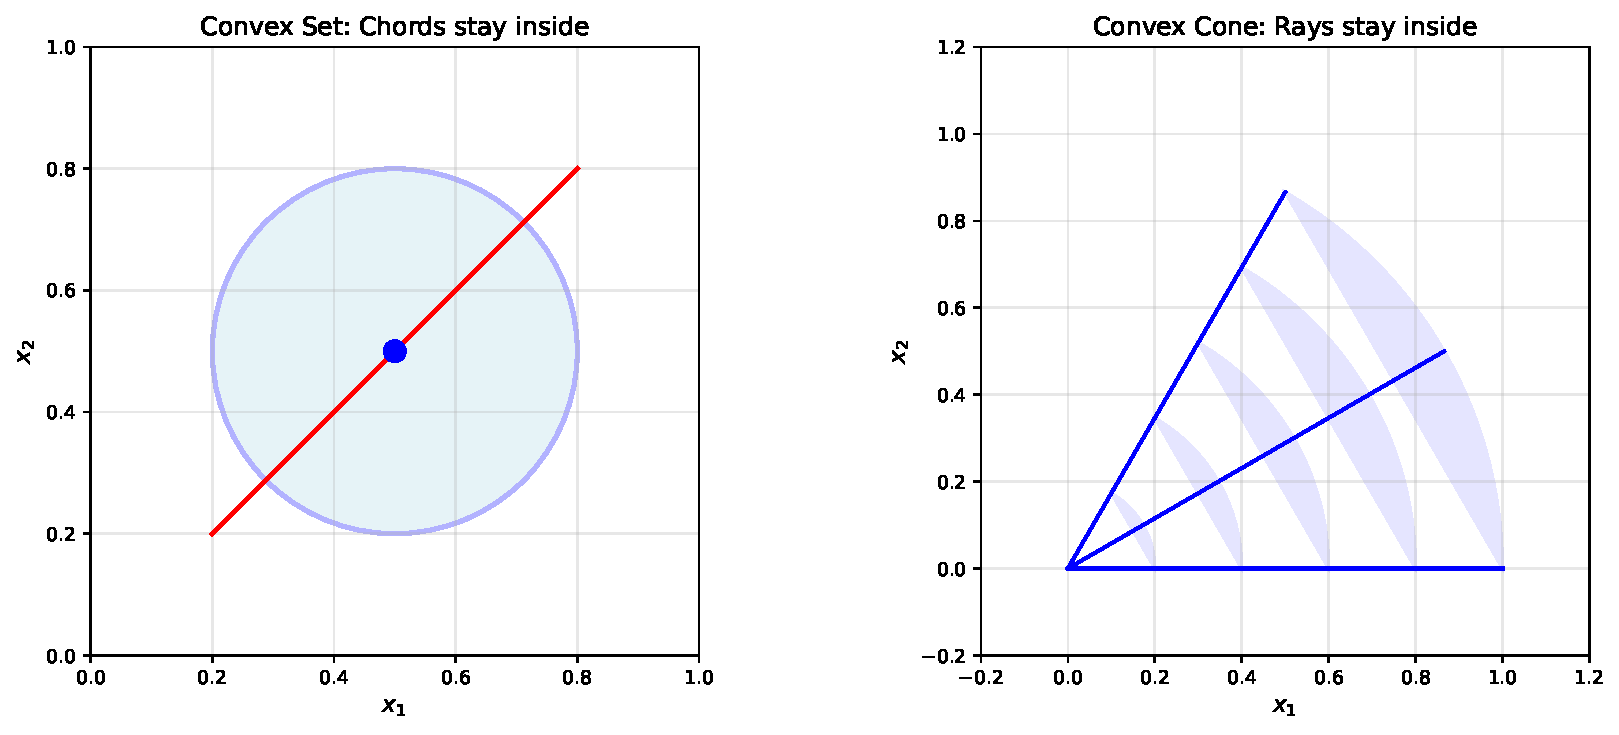
\includegraphics[width=0.9\textwidth]{convex_sets.pdf}
  
  Convex sets and cones are fundamental to understanding domain conditions in duality.
\end{frame}

% ============================================================================
% SECTION 15.4: Conjugation Result
% ============================================================================

\section[15.4]{Section 15.4: A Conjugation Result}

\begin{frame}{Theorem 15.27: Conjugate of Composite Function}
  \begin{block}{Theorem 15.27}
    Let $f \in \Gamma_0(\mathcal{H})$, $g \in \Gamma_0(\mathcal{K})$, and $L \in \mathcal{B}(\mathcal{H}, \mathcal{K})$.
    
    Suppose one of:
    \begin{enumerate}
      \item[(i)] $0 \in \text{sri}(\text{dom} g - L(\text{dom} f))$
      \item[(ii)] $\mathcal{K}$ finite-dim., $g$ polyhedral, $\text{dom} g \cap L(\text{dom} f) \neq \emptyset$
      \item[(iii)] $\mathcal{H}, \mathcal{K}$ finite-dim., $f, g$ polyhedral, $\text{dom} g \cap L(\text{dom} f) \neq \emptyset$
    \end{enumerate}
    
    Then:
    \[
      (f + g \circ L)^*(u) = \min_{v \in \mathcal{K}} [f^*(u - L^*v) + g^*(v)]
    \]
  \end{block}
  
  \vspace{0.3cm}
  \textbf{Key Formula:} The conjugate of a composite function is a constrained minimization.
\end{frame}

\begin{frame}{Corollary 15.28: Simplified Case}
  \begin{block}{Corollary 15.28}
    Let $g \in \Gamma_0(\mathcal{K})$ and $L \in \mathcal{B}(\mathcal{H}, \mathcal{K})$.
    
    Suppose one of:
    \begin{enumerate}
      \item[(i)] $0 \in \text{sri}(\text{dom} g - \text{ran} L)$
      \item[(ii)] $\mathcal{K}$ finite-dim., $g$ polyhedral, $\text{dom} g \cap \text{ran} L \neq \emptyset$
    \end{enumerate}
    
    Then:
    \[
      (g \circ L)^*(u) = L^* \circ g^*(u) = \min_{v \in \mathcal{K}, L^*v = u} g^*(v)
    \]
  \end{block}
\end{frame}

% ============================================================================
% SECTION 15.5: Applications
% ============================================================================

\section[15.5]{Section 15.5: Applications}

\begin{frame}{Application 1: Von Neumann's Minimax Theorem}
  \begin{block}{Corollary 15.30 (Von Neumann)}
    Let $C$ be a nonempty bounded closed convex subset of $\mathcal{H}$, $D$ a nonempty bounded closed convex subset of $\mathcal{K}$, and $L \in \mathcal{B}(\mathcal{H}, \mathcal{K})$.
    
    Then:
    \[
      \min_{x \in C} \max_{v \in D} \langle Lx, v \rangle = \max_{v \in D} \min_{x \in C} \langle Lx, v \rangle
    \]
  \end{block}
  
  \vspace{0.3cm}
  \textbf{Proof:} Set $f = \iota_C$, $g = \iota_D$, then:
  \[
    \min_x [f(x) + g(Lx)] = \min_x \iota_C(x) + \iota_D(Lx)
  \]
  
  Apply Fenchel-Rockafellar duality with $f^* = \sigma_C$, $g^* = \sigma_D$ (support functions).
\end{frame}

\begin{frame}{Application 2: Minimax Visualization}
  \centering
  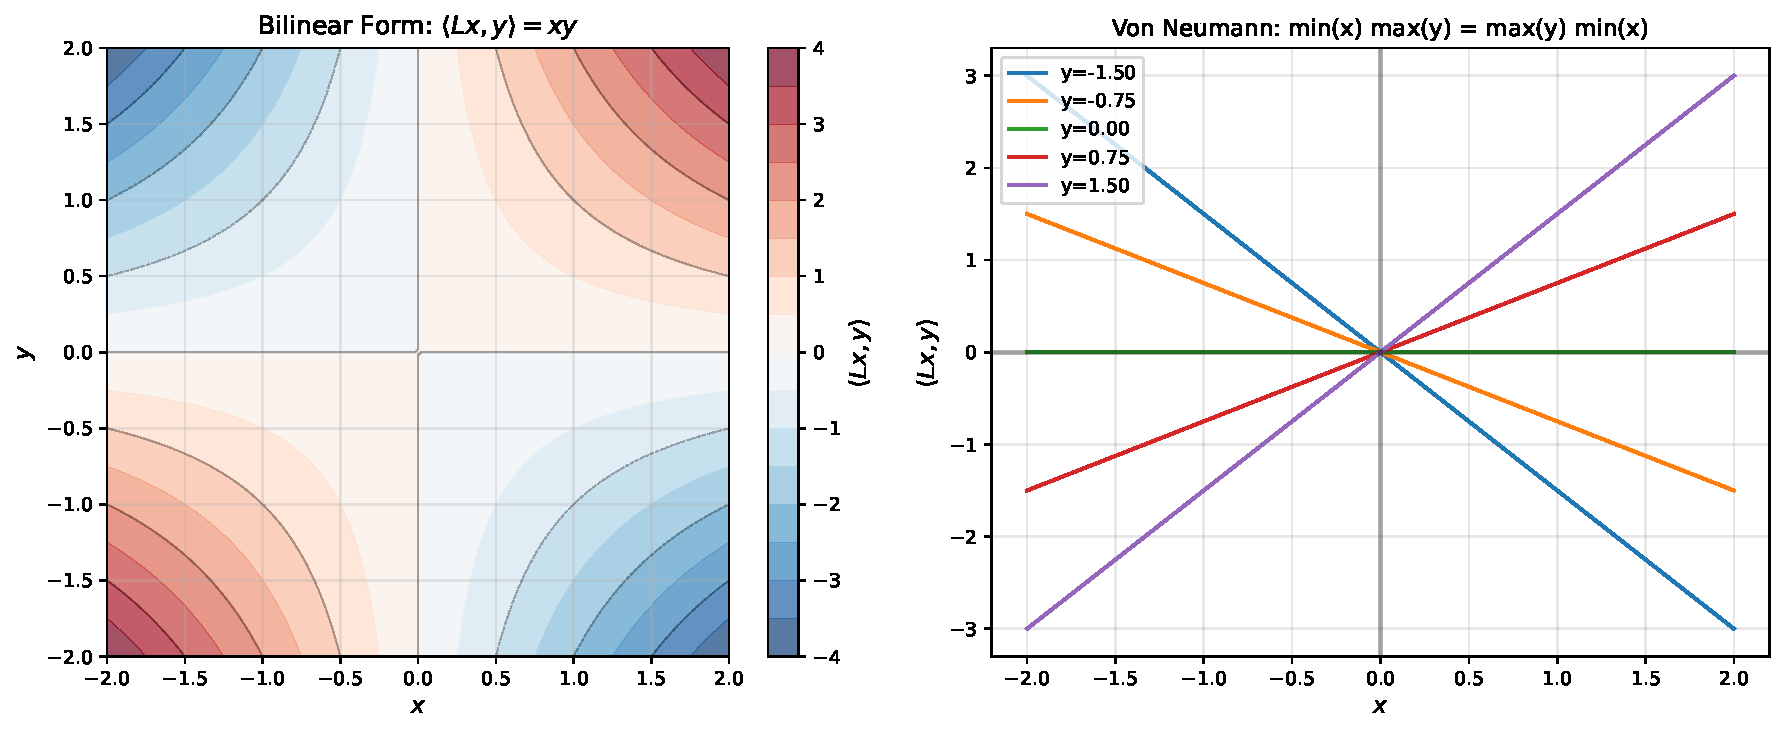
\includegraphics[width=0.95\textwidth]{minimax_theorem.pdf}
  
  Von Neumann's theorem: order of min and max can be exchanged under convexity conditions.
\end{frame}

\begin{frame}{Application 3: Conjugate Cones and Polars}
  \begin{block}{Corollary 15.31}
    Let $C, D$ be nonempty closed convex cones, and $L \in \mathcal{B}(\mathcal{H}, \mathcal{K})$.
    
    Then:
    \begin{enumerate}
      \item[(i)] $(C \cap L^{-1}(D))^\circ = C^\circ + L^*(D^\circ)$
      
      \item[(ii)] If $D - L(C)$ is closed linear subspace:
        \[
          (C \cap L^{-1}(D))^\circ = C^\circ + L^*(D^\circ) \text{ is nonempty closed convex cone}
        \]
    \end{enumerate}
  \end{block}
  
  \vspace{0.3cm}
  These results characterize closure of sums and compositions of cones.
\end{frame}

\begin{frame}{Application 4: Operator Range Closedness}
  \begin{block}{Corollary 15.34}
    Let $L \in \mathcal{B}(\mathcal{H}, \mathcal{K})$. Then $\text{ran} L$ is closed iff $\text{ran} L^*$ is closed.
  \end{block}
  
  \begin{block}{Corollary 15.35}
    Let $U, V$ be closed linear subspaces of $\mathcal{H}$. Then $U + V$ is closed iff $U^\perp + V^\perp$ is closed.
  \end{block}
  
  \begin{block}{Corollary 15.36}
    Let $L \in \mathcal{B}(\mathcal{H}, \mathcal{K})$ with closed range and $V$ a closed subspace. Then $L(V)$ is closed iff $V + \ker L$ is closed.
  \end{block}
  
  \vspace{0.3cm}
  \textbf{Impact:} These characterizations are essential in functional analysis.
\end{frame}

\begin{frame}{Key Properties Summary}
  \centering
  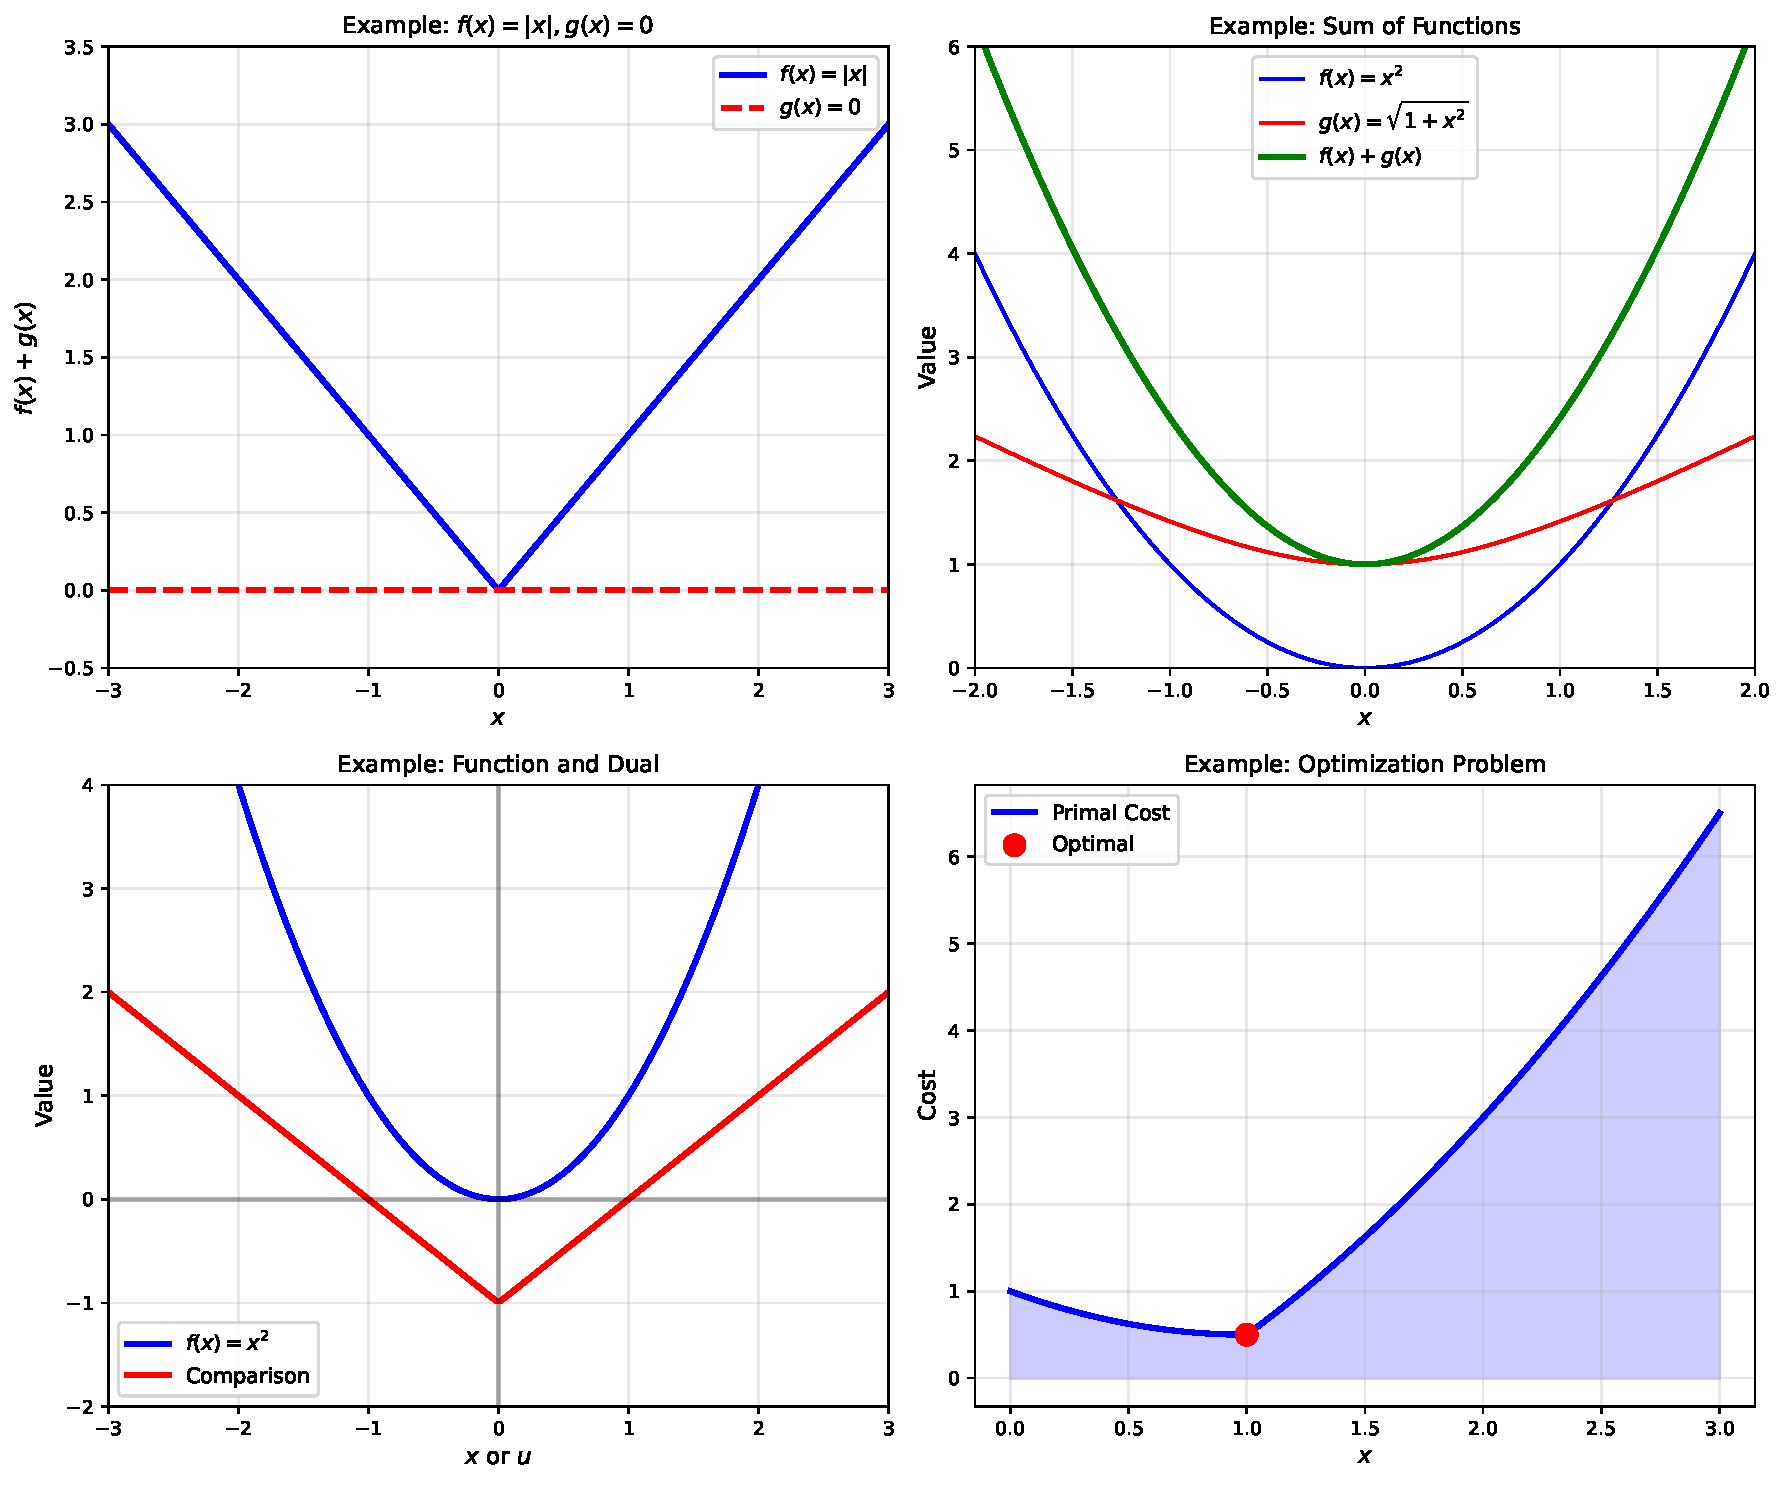
\includegraphics[width=0.95\textwidth]{examples_1d.pdf}
\end{frame}

% ============================================================================
% Numerical Examples
% ============================================================================

\section{Numerical Examples}

\begin{frame}[fragile]{Example 1: Quadratic + Absolute Value}
  \textbf{Problem:} $\min_x \left[ \frac{1}{2}\|x\|_2^2 + |x_1| + |x_2| \right]$
  
  \vspace{0.3cm}
  
  \begin{lstlisting}
import numpy as np
from scipy.optimize import minimize

# Primal problem
def objective(x):
    return 0.5*np.sum(x**2) + np.sum(np.abs(x))

x0 = np.zeros(2)
result = minimize(objective, x0, method='BFGS')
print(f"Optimal x: {result.x}")
print(f"Optimal value: {result.fun}")

# Dual conjugates:
# f(x) = 0.5||x||^2, f*(u) = 0.5||u||^2
# g(x) = |x|, g*(u) = 0 if ||u||_inf <= 1, else inf
  \end{lstlisting}
  
  \vspace{0.3cm}
  The strong duality condition is satisfied, so primal and dual optimal values are equal.
\end{frame}

\begin{frame}[fragile]{Example 2: Linear Constraint}
  \textbf{Problem:} $\min_x f(x)$ subject to $Lx = y$ (encoded in conjugate)
  
  \vspace{0.3cm}
  
  \begin{lstlisting}
import numpy as np

# Primal: min [f(x) + g(Lx)] where g = iota_{y}
# Dual: min [f*(-L*v) + g*(v)]

# Example: L is linear map, y is target
L = np.array([[1, 1], [1, -1]])
y = np.array([1, 0])

def primal_objective(x):
    residual = L @ x - y
    return np.linalg.norm(residual)**2

# Dual via Fenchel-Rockafellar:
# min_v ||L^T v||^2 / 4 + ||y - v||^2
def dual_objective(v):
    return np.linalg.norm(L.T @ v)**2 / 4 + \
           np.linalg.norm(y - v)**2
  \end{lstlisting}
\end{frame}

\begin{frame}[fragile]{Example 3: Composite Functions}
  \textbf{Computing Conjugate of $f(x) + g(Lx)$}

  \vspace{0.3cm}

  \begin{lstlisting}
import numpy as np

# Given: f, g, L
# Compute: (f + g @ L)*(u)

def conjugate_of_composite(u, f_star, g_star, L_star):
    """
    Theorem 15.27:
    (f + g @ L)*(u) = min_v [f*(u - L*v) + g*(v)]
    """
    def objective(v):
        return f_star(u - L_star @ v) + g_star(v)

    from scipy.optimize import minimize
    result = minimize(objective, np.zeros_like(u))
    return result.fun

# Example: f(x) = ||x||^2/2, g(x) = |x|, L = I
f_star = lambda u: np.linalg.norm(u)**2 / 2
L_star = np.eye(2)
  \end{lstlisting}
\end{frame}

% ============================================================================
% Summary and Conclusion
% ============================================================================

\section{Summary}

\begin{frame}{Chapter 15 Summary}
  \textbf{Major Results:}
  
  \begin{enumerate}
    \item \textbf{Attouch-Brézis:} $(f+g)^* = f^* \text{ } \square \text{ } g^*$ under domain conditions
    
    \item \textbf{Fenchel Duality:} Primal-dual framework with duality gap
      \[
        \inf(f+g) = -\inf(f^*+g^*) \text{ if } \Delta(f,g)=0
      \]
    
    \item \textbf{Fenchel-Rockafellar:} Extension with linear operators
      \[
        \inf(f + g \circ L) = -\min(f^* \circ (-L^*) + g^*) 
      \]
    
    \item \textbf{Conjugate Formula:} For composite functions
      \[
        (f + g \circ L)^*(u) = \min_v [f^*(u - L^*v) + g^*(v)]
      \]
    
    \item \textbf{Applications:}
      \begin{itemize}
        \item Von Neumann's minimax theorem
        \item Characterization of closed operator ranges
        \item Properties of convex cones and subspaces
      \end{itemize}
  \end{enumerate}
\end{frame}

\begin{frame}{Key Conditions}
  \textbf{Sufficient Conditions for Strong Duality:}
  
  \vspace{0.3cm}
  
  Most results require one of:
  \begin{enumerate}
    \item $0 \in \text{sri}(\text{dom} f - \text{dom} g)$ \quad (strong relative interior)
    \item $0 \in \text{int}(\text{dom} f - \text{dom} g)$ \quad (interior)
    \item $0 \in \text{core}(\text{dom} f - \text{dom} g)$ \quad (core)
    \item Relative interior conditions in finite dimensions
    \item Explicit finiteness and polyhedrality assumptions
  \end{enumerate}
  
  \vspace{0.3cm}
  
  \textbf{Why These Conditions?}
  \begin{itemize}
    \item Ensure properness and lower semicontinuity
    \item Guarantee exact conjugacy formulas
    \item Avoid pathological examples with duality gap
  \end{itemize}
\end{frame}

\begin{frame}{Duality Framework Visualization}
  \centering
  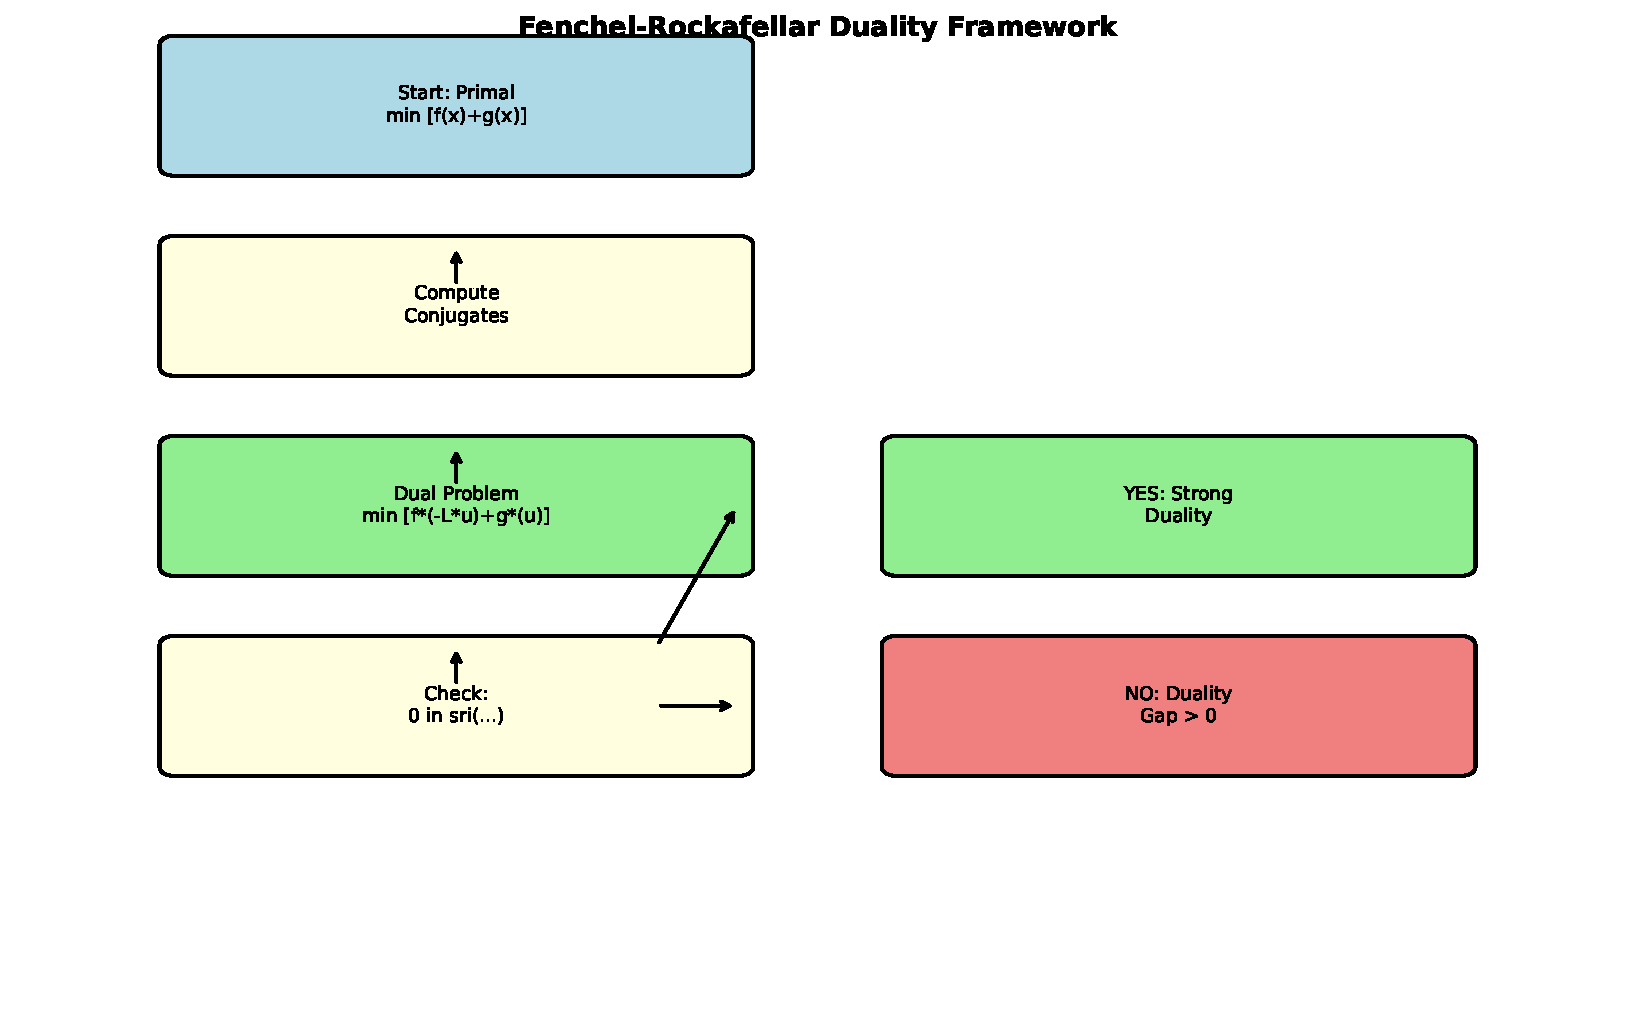
\includegraphics[width=0.9\textwidth]{algorithm_flow.pdf}
\end{frame}

\begin{frame}{Fenchel Conjugate Visualization}
  \centering
  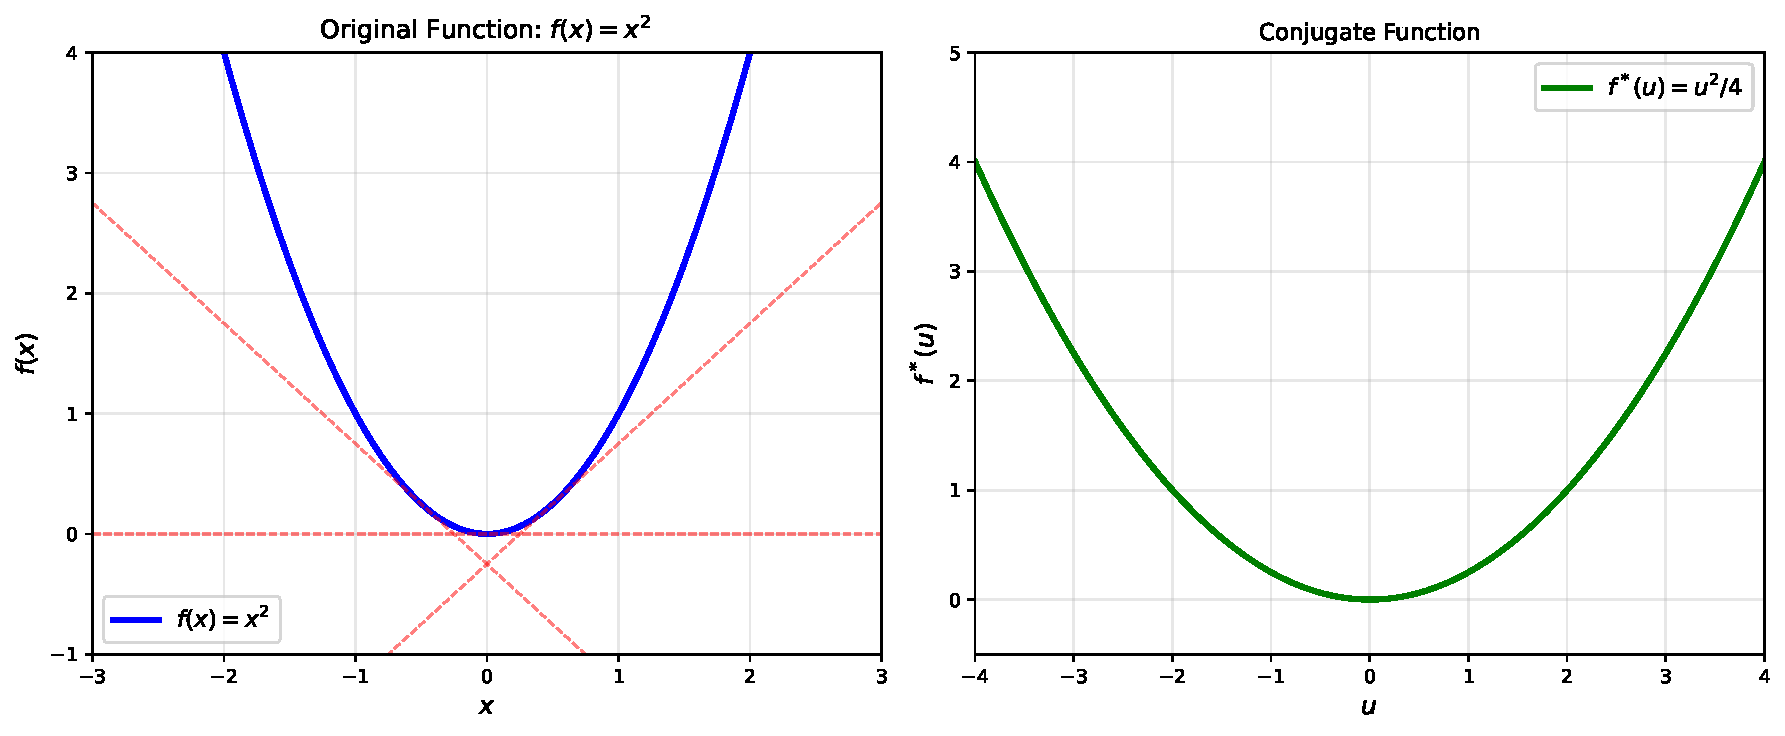
\includegraphics[width=0.95\textwidth]{fenchel_conjugate.pdf}
\end{frame}

\begin{frame}[fragile]{Computational Perspective}
  \textbf{Practical Algorithm:}
  
  \begin{lstlisting}
# Step 1: Identify primal problem structure
# min_x [f(x) + g(Lx)]

# Step 2: Check domain condition
# 0 in sri(dom g - L(dom f))?

# Step 3: Compute conjugate functions
# f*(u) = sup_x [<u,x> - f(x)]
# g*(v) = sup_y [<v,y> - g(y)]

# Step 4: Formulate dual problem
# min_v [f*(-L*v) + g*(v)]

# Step 5: Solve dual (often easier)
# Use convex optimization methods

# Step 6: Recover primal solution
# From strong duality: optimal values match
# Can extract x from v via optimality conditions
  \end{lstlisting}
  
  \vspace{0.2cm}
  This approach is fundamental in optimization algorithms.
\end{frame}

\begin{frame}{Further Reading}
  \begin{itemize}
    \item \textbf{Boyd \& Vandenberghe} (2004): Convex Optimization
      \begin{itemize}
        \item Standard reference for convex duality
      \end{itemize}
    
    \item \textbf{Rockafellar} (1970): Convex Analysis
      \begin{itemize}
        \item Foundational monograph on Fenchel duality
      \end{itemize}
    
    \item \textbf{Nesterov} (2004): Introductory Lectures on Convex Optimization
      \begin{itemize}
        \item Algorithmic perspective on duality
      \end{itemize}
    
    \item \textbf{Bauschke \& Combettes} (2011): Convex Analysis and Monotone Operator Theory
      \begin{itemize}
        \item Comprehensive treatment (this book)
      \end{itemize}
  \end{itemize}
\end{frame}

\begin{frame}
  \centering
  \Large

  \textbf{Thank you!}

  \vspace{1cm}

  Chapter 15: Fenchel-Rockafellar Duality

  \vspace{0.5cm}

  \normalsize
  Questions?
\end{frame}

\end{document}
